\chapter{Sequence models}

Next, we will implement models which take the ordering of tokens into
account. This includes \acp{CNN} and \acp{RNN}.

For the models in this chapter, we needed to set a fixed number of tokens
such that shorter documents were padded to this length, and longer documents
truncated. In order to decide this, we examined the distribution of document
lengths in the training set. All subsequent values are rounded to the nearest
integer. First, we found the 95th percentile of document lengths, which
turned out to be 701 tokens. Then, we computed the value $Q_2 + 1.5 \cdot
(Q_3 - Q_1)$, or the median plus 1.5 times the interquartile range, which
gives 693 tokens. Finally, we computed the mean value plus two standard
deviations, giving 707 tokens. These values are all close to each other, and
we decided to settle on 700 tokens since it is a round number close to all
values we examined.


\section{Convolutional neural networks}

We create a model with convolutional architecture based on the model
described in \textcite{zhang2017sensitivity}. The basis of this architecture
is a set of filter banks with varying window size. After applying the
convolutions, the output is pooled along the time axis, leaving a vector with
as many elements as there are filters in the filter banks. The vectors for
each of the filter banks are concatenated into a single vector.


\subsection{Results}

The \ac{CNN} classifier that used both tokens and POS tags as input performed
better than the one which only used tokens as input, as seen in table
\ref{tab:cnn-results}. However, on the collapsed label set, the model which only
used tokens had a higher accuracy.

\begin{table}
  \centering
  \begin{tabular}{lrrrr}
    \toprule
            & \multicolumn{2}{c}{All labels} & \multicolumn{2}{c}{Collapsed labels} \\
    \cmidrule(lr){2-3}
    \cmidrule(lr){4-5}
    Model     & Macro \FI      & Micro \FI      & Macro \FI      & Micro \FI \\
    \midrule
    Tokens    &         $0.234$  &         $0.415$  &         $0.423$  & $\mathbf{0.797}$ \\
    +POS      & $\mathbf{0.283}$ & $\mathbf{0.431}$ & $\mathbf{0.444}$ &         $0.772$  \\
    \bottomrule
  \end{tabular}
  \caption{\FI scores of CNN classifiers on AES}
  \label{tab:cnn-results}
\end{table}


\section{Recurrent neural networks}

A \ac{LSTM} \ac{RNN} was implemented based on the architecture described by
\textcite{taghipour16}. Several changes to their architecture were made in
order to accomodate our data. For instance, \citeauthor{taghipour16} modelled
the task as a regression problem, their output layer consisting of a single
node with a value constrained to (0, 1) by the sigmoid function. This layer
was replaced with a softmax layer similar to the \acp{MLP} in section
\ref{subsec:mlp}. The loss function needed to be compatible with a
multi-class softmax output. We used categorical cross-entropy. A different
evaluation metric was also needed because we are treating the task as
multi-class prediction. We are reporting macro and micro \FI as before. The
\ac{QWK} metric used by \citeauthor{taghipour16} is not applicable to the
predictions of our classifier.

The embedding layer in \textcite{taghipour16} was initialized with
pre-trained embeddings of size 50. Our embedding layer was initialized to
random vectors and trained as part of the network.

Unlike our corpus, ASK, the dataset used by \citeauthor{taghipour16}
contained essays that were not necessarily written in a second language. Our
data is not split into different parts based on the prompt. There are two
different test levels in ASK, but these are not distinguished in training.

where $\sigma$ by default in Keras is the \emph{Hard sigmoid} activation
function, chosen because it is computationally more efficient than the
sigmoid function, and defined in equation \ref{eq:hardsigmoid}.

We also experimented with a different type of \ac{RNN} cell, the \ac{GRU}.
This variant of \ac{RNN} is slightly simpler than the \ac{LSTM}, featuring
only two gates. However, it is still designed to be able to propagate the
error gradient over a larger number of timesteps and is supposed to solve the
same problems as \ac{LSTM}. The equations defining a \ac{GRU} layer are
defined in equation \ref{eq:gru}:



\subsection{Variants}

We attempt two different methods of combining the sequence of hidden states
from the \ac{LSTM} into a feature vector. The simplest approach is \emph{mean
over time}, where we use the elementwise average of elements in hidden states
across the time dimension as our feature vector. The mean over time layer is
used in two of the experiments. Once with a \ac{LSTM} processing the essay
from top to bottom, and once on top of a bidirectional LSTM (BiLSTM). In the
BiLSTM, the output from the \ac{RNN} on each timestep is the concatenation of
the states of two \acp{LSTM}, one processing the document from the top and
the other one from the bottom up.

\todo{A paragraph on BiLSTM} The bidirectional model is constructed by
running two \acp{LSTM} over the same input, but in the opposite order. The
output from the BiLSTM layer is a sequence of vectors where, for each
timestep $j$, the vector is the concatenation of the output from the forwards
\ac{LSTM} after processing the inputs $(x_1, x_2, \ldots, x_j)$ and the
output from tha backwards \ac{LSTM} after processing the inputs $(x_m,
x_{m-1}, \ldots, x_j)$, $m$ being the total number of timesteps. The BiLSTM
should therefore be able to extract context on both sides of a input
timestep.

\todo{Mean of the final state}
\todo{Add POS inputs to RNN}
\todo{GRU cells}

The attention model uses an attention layer, which instead computes a
weighted sum of the states, and therefore should be able in theory to
disregard uninformative timesteps and improve performance. In order to find
the weight to apply to each state, a single-layer neural network computes a
value between -1 and 1 for each timestep. These values are normalized by a
softmax layer and then used to compute the weighted average. The attention
mechanism is trained along with the rest of the network. The attention model
uses a unidirectional \ac{LSTM}.

The modified model differs in which parts of the network uses dropout, as
well as in certain hyperparameters. All the models use word embedding vectors
of size 50 and a hidden state vector of size 300 in the \ac{LSTM}. The
vocabulary was limited to the 4,000 most common words.


\subsection{Results}

Results for four different models are shown in table \ref{tab:lstm-results}. All
but \emph{Modified} are using the same hyperparameters as
\citeauthor{taghipour16}. The \emph{Attention} model does not use masking,
while \emph{Mean/Time} and \emph{BiLSTM} do.
\todo{Always use pre-trained embeddings when repeating the experiments?}

\begin{table}
  \centering
  \begin{tabular}{lrrrr}
    \toprule
            & \multicolumn{2}{c}{All labels} & \multicolumn{2}{c}{Collapsed labels} \\
    \cmidrule(lr){2-3}
    \cmidrule(lr){4-5}
    Model     & Macro \FI      & Micro \FI      & Macro \FI      & Micro \FI \\
    \midrule
    % 50 dim, pretrained, fine tune
    %
    Mean/Time &         $0.280$  &         $0.382$  &         $0.461$  &         $0.699$  \\
    %           taghipour_ng-2019-01-22_12-58-00      taghipour_ng-2019-01-22_13-01-44
    BiLSTM    &         $0.286$  &         $0.398$  &         $0.485$  &         $0.683$  \\
    %           taghipour_ng-2019-01-24_19-16-41      taghipour_ng-2019-01-24_21-23-34
    Attention & $\mathbf{0.303}$ &         $0.423$  & $\mathbf{0.558}$ & $\mathbf{0.805}$ \\
    \midrule
    % 100 dim, pretrained, fine tune
    %
    Mean/Time &         $0.280$  &         $0.382$  &         $0.461$  &         $0.699$  \\
    %
    BiLSTM    &         $0.286$  &         $0.398$  &         $0.485$  &         $0.683$  \\
    %
    Attention & $\mathbf{0.303}$ &         $0.423$  & $\mathbf{0.558}$ & $\mathbf{0.805}$ \\
    \bottomrule
  \end{tabular}
  \caption{\FI scores of LSTM classifiers}
  \label{tab:lstm-results}
\end{table}

The attention model performs best. While the modified model has the highest
micro \FI, the stopping criterion is based on the macro \FI, and the micro \FI
scores are not necessarily comparable\textemdash the ranking of models might
be different if the stopping criterion was mased on micro \FI instead of
macro.

\todo{Analysis of attention model}
\todo{Per-class results}


\section{Native language identification}

We train the same models to classify the documents by native language. The
performance of a \ac{CNN} model improved drastically when including \ac{POS}
tags as input, as evident in table \ref{tab:cnn-nli-results}.

The \ac{RNN} model was able to achieve even better performance, and we still
see that the attention model outperforms the rest.

\begin{table}
  \centering
  \begin{tabular}{lrr}
    \toprule
    Model     & Macro \FI      & Micro \FI \\
    \midrule
    Tokens    &         $0.367$  &         $0.366$  \\ % cnn-nli-2019-02-05_12-54-51
    +POS      & $\mathbf{0.467}$ & $\mathbf{0.463}$ \\ % cnn-nli-2019-01-30_15-32-28
    \bottomrule
  \end{tabular}
  \caption{\FI scores of CNN classifiers on NLI}
  \label{tab:cnn-nli-results}
\end{table}

\begin{table}
  \centering
  \begin{tabular}{lrr}
    \toprule
    Model     & Macro \FI      & Micro \FI \\
    \midrule
    Mean/Time &         $0.379$  &         $0.390$  \\ % rnn_nli-25740792
    BiLSTM    &         $0.468$  &         $0.480$  \\ % rnn_nli-25740786
    Attention & $\mathbf{0.423}$ & $\mathbf{0.407}$ \\ % rnn_nli-25740789
    \bottomrule
  \end{tabular}
  \caption{\FI scores of RNN classifiers on NLI}
  \label{tab:rnn-nli-results}
\end{table}
\todo{Include POS in RNN models}

The attention model allows us to visualize the weights the network gives to
each token in a document. Figure \ref{fig:nli-attention} shows the first 300
tokens of a text which was correctly predicted to be written by a native Polish
speaker. Red tokens indicate timesteps that were given higher weight by the attention
model, and blue tokens ones that were given low weights. Out of vocabulary tokens
are replaced by question mark emoji. The attention values do not seem easily
interpretable, as there are lexical and grammatical errors both in the red and
the blue sections.

\begin{figure}
  \centering
  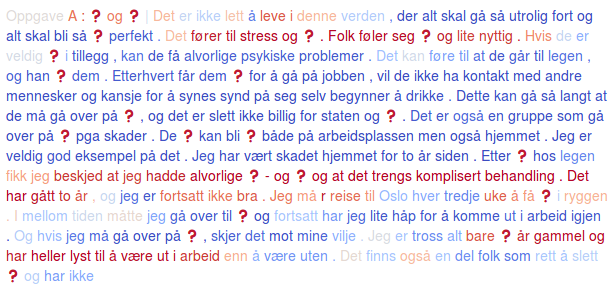
\includegraphics[width=\textwidth]{nli-attention}
  \caption{Attention values of NLI classifier on excerpt from ASK text h0131}
  \label{fig:nli-attention}
\end{figure}
